\chapter[W Bosons]{W Bosons at the LHC}
\label{chap:wboson}

\PW boson production is an important process for physics studies at the LHC.  At
the \ac{LHC}, \PW bosons are produced at a high rate while offering a clean
experimental signal with a final state consisting of, in the case of a
leptonically decaying \PW, a single high \PT lepton with a large amount of
missing transverse energy due to the neutrino in the event. 
\todo{reread this}

The production of \PW, through the \ac{DY} process, provides important
information on the interacting partons within the colliding hadrons.

\section{W Boson Production}

The dominant production process for a \PW boson at a proton-proton collider is
shown in \EquationRef{wbos:wprod},

\begin{equation}
  h_1(p_1) + h_2(p_2)
  \to 
  \PW + X
  \to
  \Plepton \Pnue + X.
  \label{wbos:wprod}
\end{equation}

\begin{figure}[htbp]
  \centering
  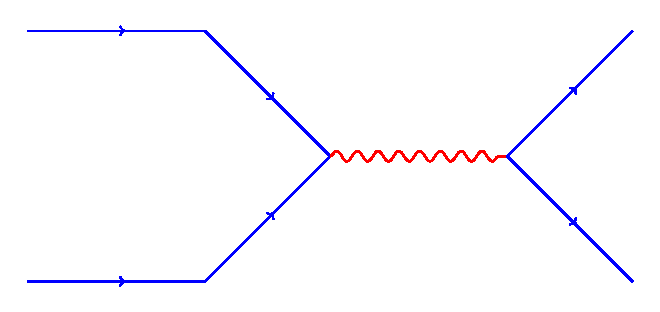
\includegraphics[width=0.8\textwidth]{w_production}
  \caption{Diagram of a W boson production and leptonic decay at a hadron-hadron collider.}
  \label{wbos:wproddiag}
\end{figure}

This process is shown in \FigureRef{wbos:wproddiag}. 
The \PW boson is produced by the collision of the two incoming hadrons $h_1$
and $h_2$ with momenta $p_1$ and $p_2$. 
$X$ represents the accompanying final state.

At proton-proton colliders the full \PW production cross section is a
convolution of the cross-section at the parton level, and the proton \ac{PDF},

\begin{multline}
  d\sigma_{(\HepProcess{h_1 h_2 \to \PWpm})}(p_1,p_2) = \\
  \sum\limits_{a,b}
  \int_0^1 \! \mathrm{d} x_1 
  \int_0^1 \! \mathrm{d} x_2 
  f_a^{h_1}(x_1,Q^2)
  f_b^{h_2}(x_2,Q^2) 
  d\hat{\sigma}_{(\HepProcess{a b \to \PWpm})}(x_1 p_1, x_2 p_2; Q^2),
  \label{wbos:xsec}
\end{multline}
where $\sum\limits_{a,b}$ represents the sum over the initial parton states $a$
and $b$, $f_a^{h}(x,Q^2)$ represents the proton \ac{PDF} and
$d\hat{\sigma}_{(\HepProcess{a b \to \PWpm})}(x_1 p_1, x_2 p_2; Q^2)$
represents the partonic sub-process cross-section.

\subsubsection*{Partonic Sub-Process}

At \ac{LO} the process for a \PWp is
\begin{equation}
  \HepProcess{\Pup + \APdown \to \PWp \to \Pleptonplus \Pnulepton} 
  \label{wbos:wpprod} 
\end{equation}
and for a \PWm:
\begin{equation}
  \HepProcess{\APup + \Pdown \to \PWm \to \Pleptonminus \APnulepton}
  \label{wbos:wmprod} 
\end{equation}

\begin{figure}[htbp]
  \centering
  \begin{subfigure}{0.45\textwidth}
    \centering
    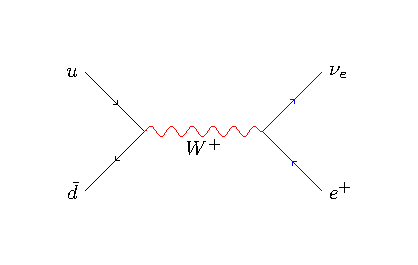
\includegraphics[width=\textwidth]{w_process_wp}
    \caption{\HepProcess{\Pup + \APdown \to \PWp \to \Pleptonplus \Pnulepton}}
    \label{fig:w_process_wp}
  \end{subfigure}
  \begin{subfigure}{0.45\textwidth}
    \centering
    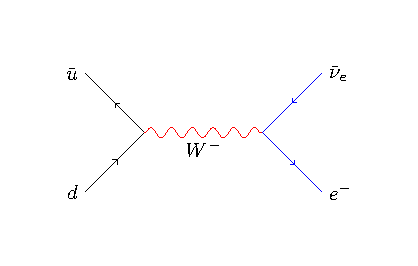
\includegraphics[width=\textwidth]{w_process_wm}
    \caption{\HepProcess{\APup + \Pdown \to \PWm \to \Pleptonminus \APnulepton}}
    \label{fig:w_process_wm}
  \end{subfigure}
  \caption{Tree-level diagrams for \PWp and \PWm boson production and electronic
decay at a hadron-hadron collider.}\label{fig:w_process} 
\end{figure}

A tree-level Feynman diagrams representing these processes are shown in
\FigureRef{fig:w_process}.
At the \ac{LHC} (a proton-proton collider), one parton is most to likely be a
valence quark with a high fraction of the proton's momentum, and the other
parton will tend to be a sea anti-quark with a lower fraction of the momentum
than the quark. The difference in momentum of the partons causes the \PW bosons 
to tend to be produced at high rapidities. 
\todo{define rapidities}

\subsubsection*{Proton \acl{PDF}} 
The proton \ac{PDF} represents the number density of parton $a$ that has a momentum
fraction $x+\mathrm{d}x$ of the colliding hadron $h$.  
\todo{describe pdfs, why a function of x and q2}


\begin{figure}[htbp]
  \centering
  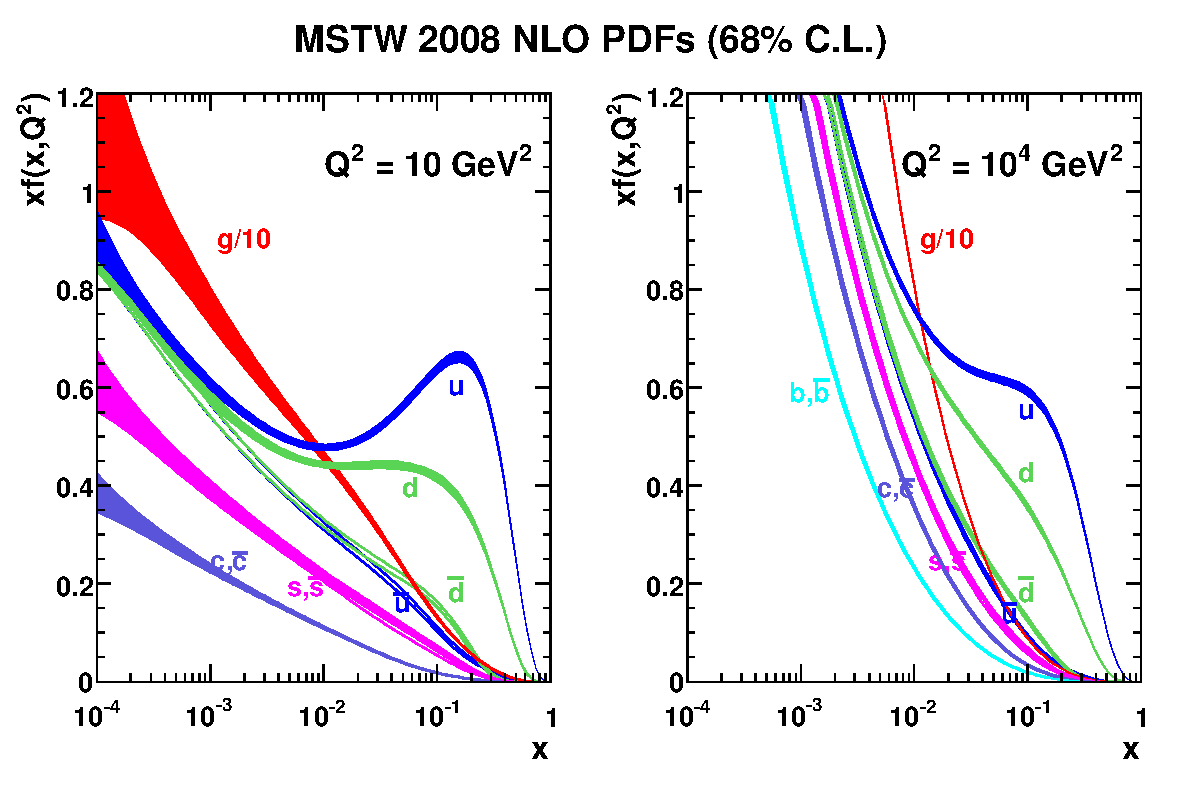
\includegraphics[width=\textwidth]{mstw2008nlo68cl_allpdfs}
  \caption{Proton PDF at  $ Q^2 = \unit{ 10  }{\GeV^2} $ (left) 
                      and $ Q^2 = \unit{ 100  }{\GeV^2} $ (right) 
                     from \cite{Martin:2009iq}. }
  \label{wbos:pdf}
\end{figure}

\acp{PDF} are obtained
from global fits to experimental data.\cite{Martin:2009iq} %TODO more?
\FigureRef{wbos:pdf} shows the proton PDF at $Q^2\approx M_{\PW}^2$ from the
MSTW group.
The anti-quark parton densities $\APup(x,Q^2)$ and $\APdown(x,Q^2)$ are
relatively similar especially at the LHC energies, where the parton momentum
fraction, x, tends to be small.

The \ac{PDF} for the valence quarks in the proton differ, the up-type quark
dominates over the down-type. This is mainly due to the valence quark content
of the proton (\HepProcess{\Pup\Pup\Pdown}).  This can be seen in the
ratio of the up-type and the down-type \acp{PDF},
\begin{equation}
  R_{ud}(x,Q^2) = \frac{\Pup(x,Q^2)}{ \Pdown(x,Q^2)} > 1,
\end{equation}
where $\Pup(x,Q^2)$ are the up and down quark \acp{PDF}.  
The ratio $R$ is a function of $x$, $R \approx 1$ for $x \ll 1$ and increases
monotonically as $x$ increases.  
\todo{ why is this not a flat ratio? }

\begin{figure}[htbp]
  \centering
  \begin{subfigure}{\textwidth}
    \centering
    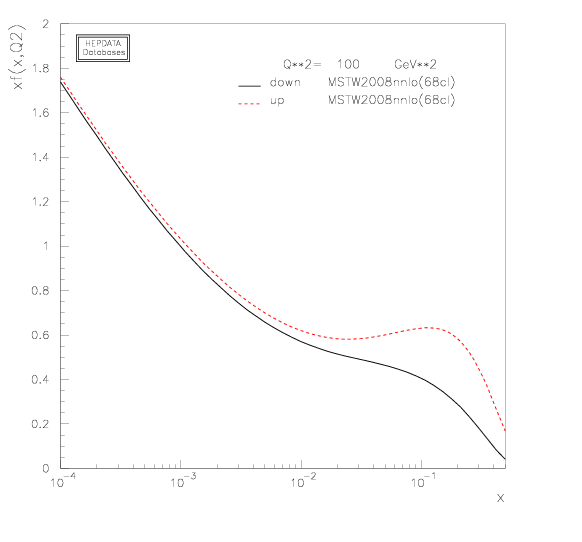
\includegraphics[width=0.75\textwidth]{plot_pdf}
    \caption{PDF for \Pup and \Pdown}
    \label{fig:plot_pdf}
  \end{subfigure}
  \begin{subfigure}{\textwidth}
    \centering
    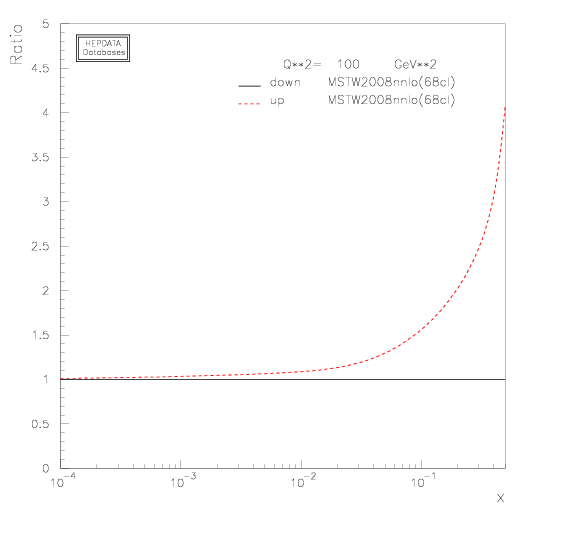
\includegraphics[width=0.75\textwidth]{plot_pdf_ratio}
    \caption{Ratio for \Pup and \Pdown PDF}
    \label{fig:plot_pdf_ratio}
  \end{subfigure}
  \caption{Ratio of up quarks to down quarks, $R_{ud}$ $ Q^2=\unit{100}{\GeV^2}$.
           Generated from \cite{}.}
  \label{fig:w_process} 
\end{figure}

\subsection{\PW Boson Rapidity Distribution}
\label{wbos:wrapsec}

The rapidity distributions for \PWp and \PWm at the \ac{LHC} are shown in
\FigureRef{wbos:wrapid}. 
The \PWm distribution is shown in the left panel and the \PWp distribution is
shown in the right panel. The distributions are invariant with respect to the
flipping the rapidity, $y\leftrightarrow-y$, so are shown on a folded rapidity
axis.
%TODO make that make sense.

\begin{figure}[htbp]
  \centering
  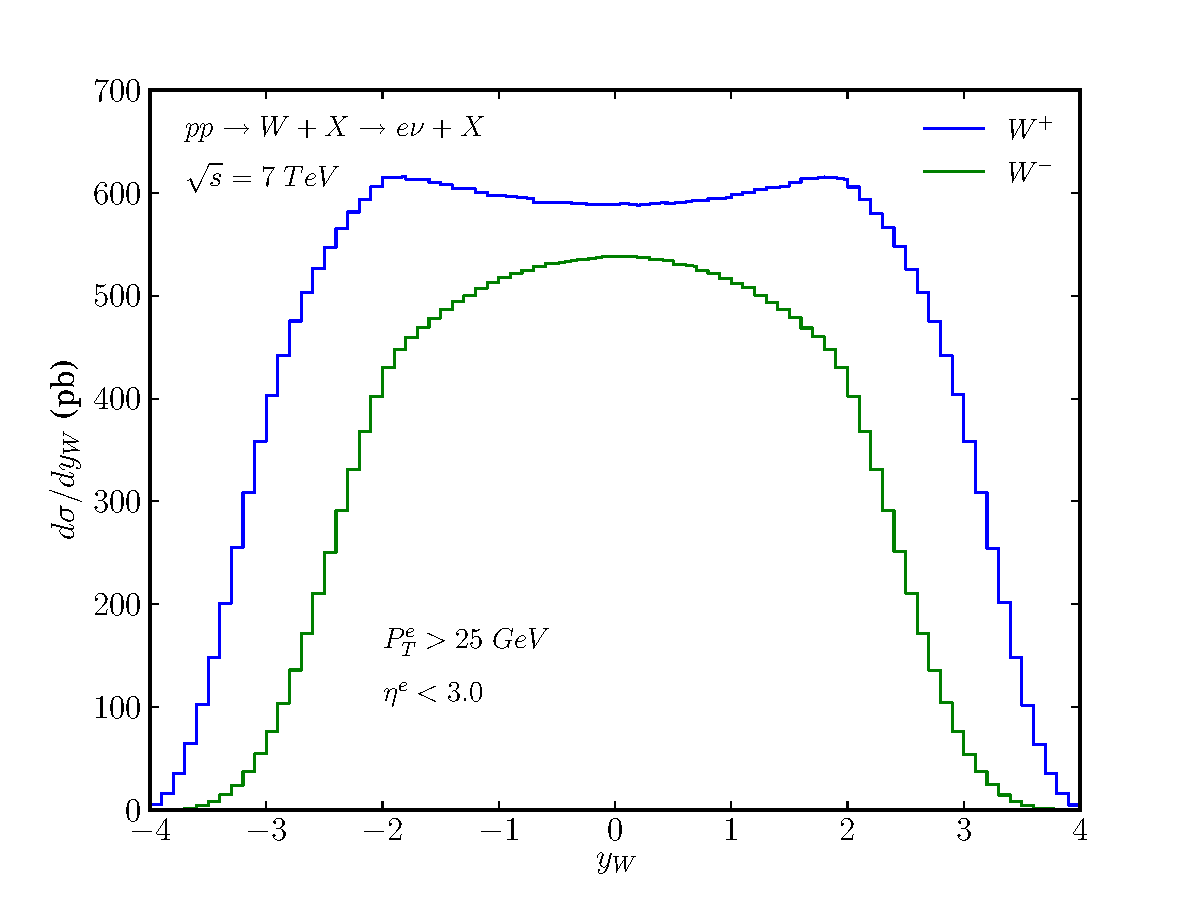
\includegraphics[width=0.8\textwidth]{w-rapidity}
  \caption{The rapidity distribution for \PWp and \PWm at the LHC.}
  \label{wbos:wrapid}
\end{figure}

In \FigureRef{wbos:wrapid} the \PWp cross section is greater than the \PWm
cross section. This is a consequence of the different production processes for
\PWp (\EquationRef{wbos:wpprod}) and \PWm (\EquationRef{wbos:wmprod}) and the
\ac{PDF} for the valence quarks in the proton differing as seen in
\FigureRef{wbos:pdfrat}. The up-type quark \ac{PDF} dominates over the
down-type which leads to a greater \PWp production rate than \PWm.

It is also seen in \FigureRef{wbos:wrapid} that the \PWm tends to be produced
more centrally whereas the \PWp is produced at larger rapidities. This is due
to \Pup quarks tending to carry a greater fraction of the proton's momentum,
$x$, than the \Pdown type quarks as seen in \FigureRef{fig:pdfrat}.

The momentum fraction, $x$, of the interaction quarks is correlated
with the rapidity of the \PW boson. The ratio of $\Pup$ and $\Pdown$ quarks as
a function of momentum fraction, $x$, is directly related to the difference in
cross-sections for \PWp and \PWm production as a function of the boson
rapidity.

Therefore a measurement of the asymmetric production of \PW bosons, as a
function of the rapidity of the boson, at the \ac{LHC} provides important
information on the ratio of the up-type and down-type quark parton densities as
a function of $x$,
$R_{ud}(x,Q^2)$, within the proton. 

\subsection{\PW Boson Charge Asymmetry}

% formalised def of w asymmetry
The \PWpm boson charge asymmetry is defined as,
\begin{equation}
  A_{W}(y_{\PW})=
    \frac{ 
      \nicefrac{ d\sigma (\PWp) }{ dy_{W} } -
      \nicefrac{ d\sigma (\PWm) }{ dy_{W} }
    }
    {
      \nicefrac{ d\sigma (\PWp) }{ dy_{W} } +
      \nicefrac{ d\sigma (\PWm) }{ dy_{W} }
    }
,
\label{wbos:wasym}
\end{equation} 
where $y_{W}$ is the boson rapidity, and 
$\nicefrac{ d\sigma (\PWpm) }{ dy_{W} }$ is the \PWpm production cross section
at a fixed $y_{W}$.  
If $d\sigma(\PWp) > d\sigma(\PWm) $ then $A_{W}(y_{\PW})> 0$,
else if $d\sigma(\PWp) < d\sigma(\PWm) $ then $A_{W}(y_{\PW})< 0$,
and for symmetric \PWpm boson production, $A_{W}(y_{\PW})= 0$,

The prediction for the W boson charge asymmetry as a function of the boson
rapidity is shown in \FigureRef{wbos:chargeasym}. $A_{W}(y_{\PW})> 0$ and
increases as the rapidity increases.

\begin{figure}[htbp]
  \centering
  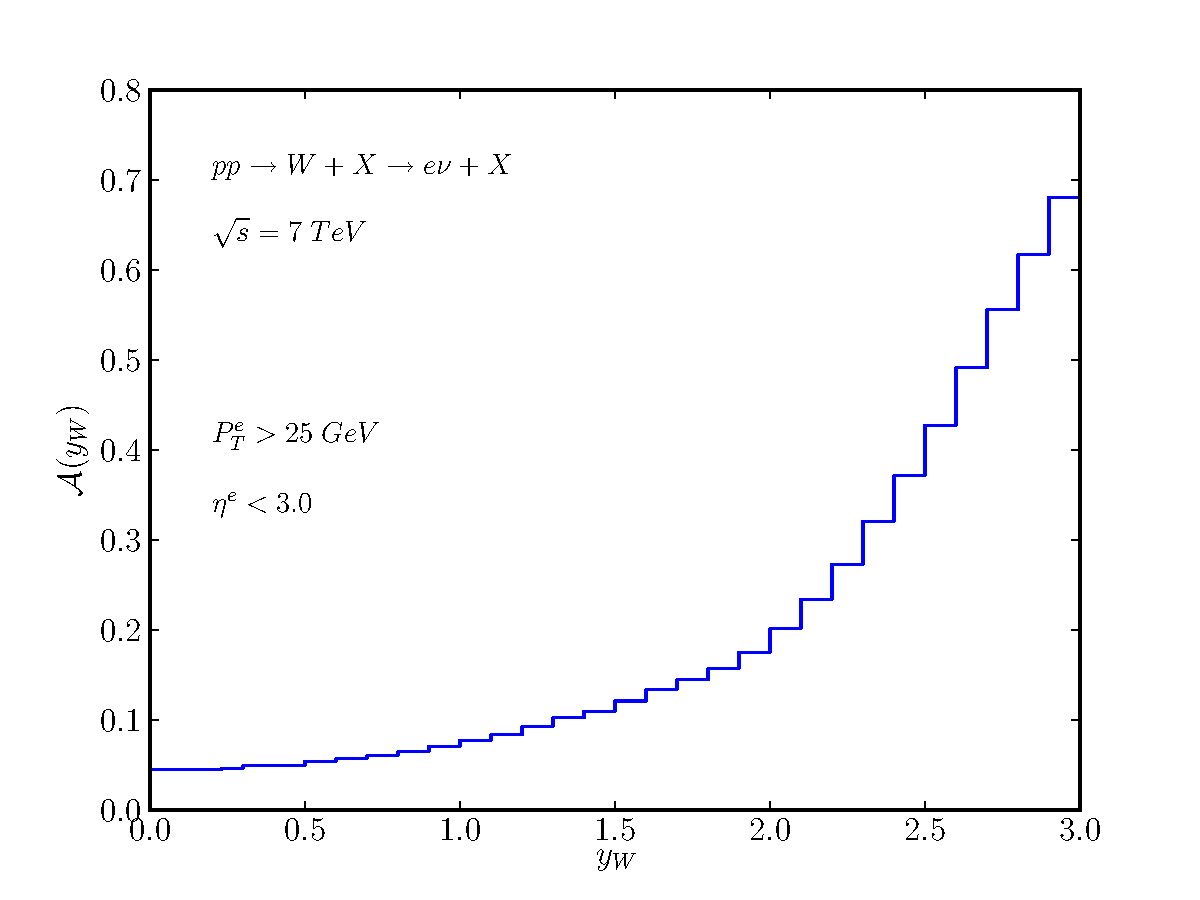
\includegraphics[width=0.8\textwidth]{w-asym}
  \caption{\PW boson charge asymmetry at LHC.}
  \label{wbos:chargeasym}
\end{figure}

\PW bosons are identified by their decay to a lepton plus neutrino, however at
hadronic colliders the neutrino longitudinal momentum cannot be determined
which means that the \PW rapidity, $y_{W}$, cannot be measured.  Instead what
is studied is the charge asymmetry in the leptons that result from the \PW boson
decaying leptonically.

%It is possible to overcome the difficulty in determining the boson rapidity
%by extrapolating the neutrino longditudinal momentum from the lepton neutrino
%with a \ac{MC} study. 

\section{W boson decay}
\todo[inline]{describe ways in which the boson can decay}
\subsection{Electron Rapidity Distribution}
The rapidity distributions of the charged lepton produced from \PW decay are
further complicated by the charge asymmetric decay of the \PWpm boson. 
The asymmetric decay arises due to the $V-A$ coupling of the \PW boson to the
annihilating \HepProcess{\Pquark\APquark} pair and the decaying lepton pair.

At \ac{LO} the \PWp is produced in the annihilation of a \Pup valance quark
with a \APdown sea-quark (\EquationRef{wbos:wpprod}). 
If the parton masses are neglected the \Pup is left-handed and the \APdown is
right-handed, as shown at the top of \FigureRef{wbos:wspin}. 
\todo{Some confusion here between helicity and handedness.}

In the \PWp decay the \Ppositron is right-handed and the \Pnue is left-handed.
\FigureRef{wbos:wspin} shows if the  positron is produced in the same direction
as the incoming \APdown quark angular momentum is conserved and the decay is
allowed.
However the decay where the positron is produced in the same direction as the
incoming \Pup quark is forbidden.
A similar argument holds true for \PWm decays, where the \Pelectron is produced
preferentially in the direction of the \Pdown.

\begin{figure}[htbp]
  \centering
  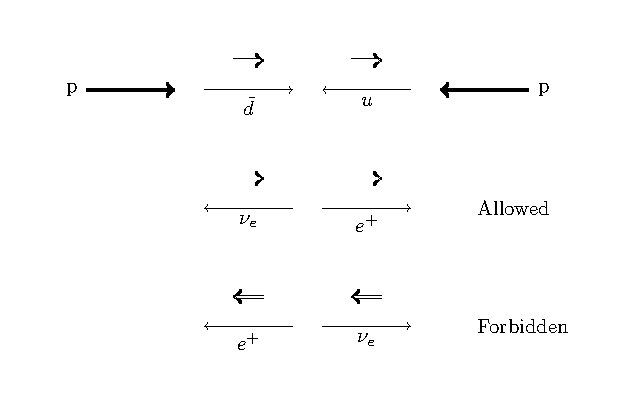
\includegraphics[width=0.8\textwidth]{w_decay_directions}
  \caption{Preferred directions of electrons in 
    \HepProcess{\PWplus\to\APelectron\Pnue} decay.}
  \label{wbos:wspin}
\end{figure}

The actual distribution of the electron from \PWpm decay in the massless limit
is given by\cite{} \todo{are we sure about this?}

\begin{equation}
  \frac{1}{\sigma_{U\bar{D}}}
  \frac{d \sigma_{U\bar{D}}}{d \cos \theta_{\Plepton D}^{\ast}}
  =
  \frac{1}{\sigma_{D\bar{U}}}
  \frac{d \sigma_{D\bar{U}}}{d \cos \theta_{\Plepton D}^{\ast}}
  =
  \frac{3}{8}(1+\cos \theta_{\Plepton D}^{\ast})^2
  \label{wbos:lepton}
\end{equation}
where $\theta_{\Plepton D}^{\ast}$ is the scattering angle of the charged
lepton with respect to the direction of the down-type quark or anti-quark, in
the centre of mass system of the two quarks. The cross-section is maximised when
$\theta_{\Plepton D}^{\ast}$ is minimised and the charged lepton is produced in
the same direction as the down-type quark.

The rapidity distribution of the electron is therefore a convolution of the
\ac{EWK} correlations in \EquationRef{wbos:lepton} with the \PW rapidity
described in \SectionRef{wbos:wrapsec},
\begin{equation}
  y_{\Plepton} = 
  y_{\PW} +
  \frac{1}{2}
  \ln
  \frac{1 + \cos \theta_{\Plepton D}^{\ast}}{1 - \cos \theta_{\Plepton D}^{\ast}}
  \label{wbos:leptonfull}
\end{equation}
\todo{I'm not sure about this, reference is needed, or leave it out}

In proton-proton collisions the \PWp tends to be produced in the direction
of the \Pup, as described in the preceding chapter.  
However, due to the EWK correlations the charged lepton from the decaying \PWp
will tend to be produced along the direction of the down type quark and
therefore will shift the rapidity distribution of the lepton to be more
central. Similarly, \PWm bosons tend to be produced more centrally, however the
EWK correlations will shift the charge lepton rapidity distribution to higher
rapidities.

\begin{figure}[htbp]
  \centering
  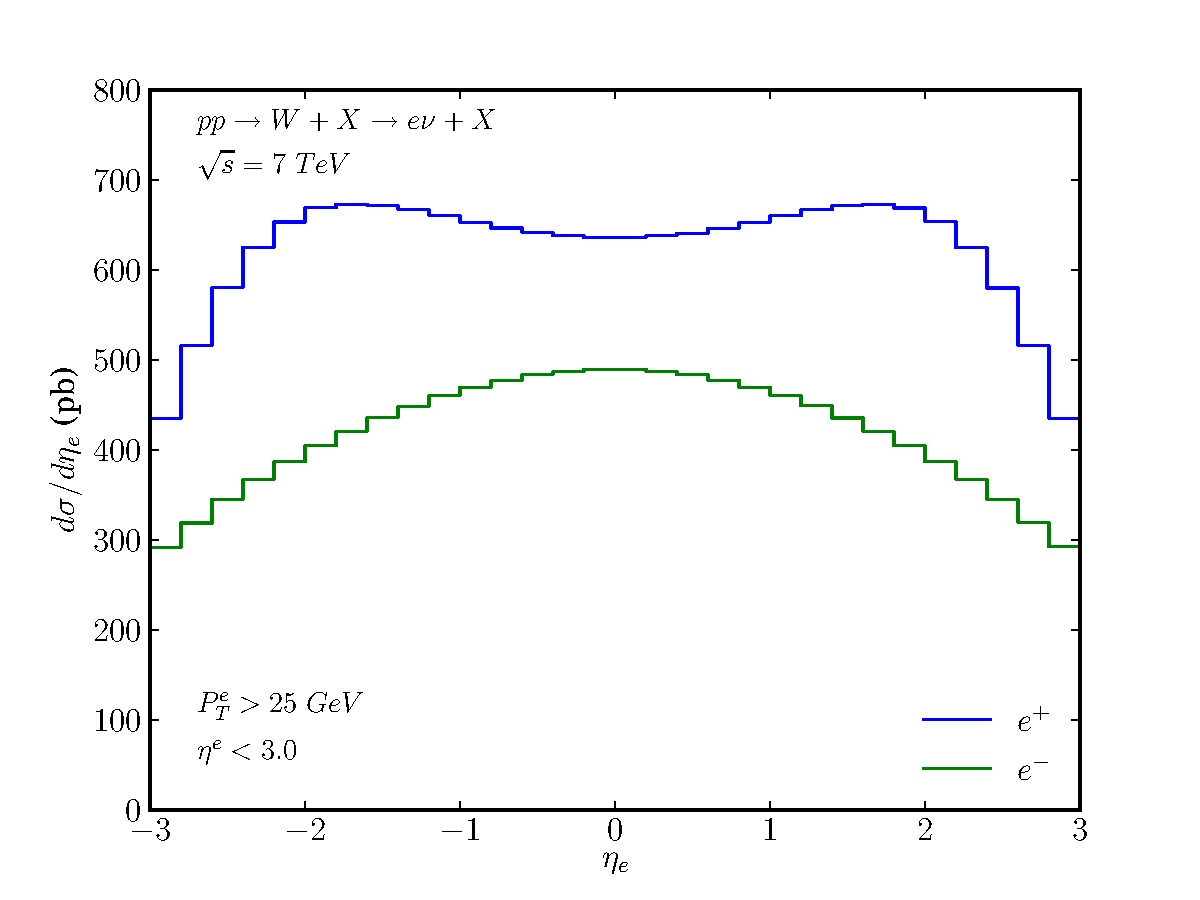
\includegraphics[width=0.8\textwidth]{lepton-rapidity}
  \caption{Electron and positron rapidity distributions.}
  \label{wbos:leptonrapidity}
\end{figure}

\subsection{Electron Charge Asymmetry}

The electron asymmetry is defined in \EquationRef{eq:AsymThe} analogously to the
\PW boson asymmetry in \EquationRef{wbos:wasym}, as the difference in the
\HepProcess{\PWplus \to \APelectron} and \HepProcess{\PWminus \to \Pelectron}
over the total \inclusiveWe cross-section.
\begin{equation}
A_{the}(\eta)=\frac{  \frac{d\sigma}{d\eta}(\Wpenu) -
\frac{d\sigma}{d\eta}(\Wmenu) }{ \frac{d\sigma}{d\eta}(\Wpenu) +
\frac{d\sigma}{d\eta}(\Wmenu) }
\label{eq:AsymThe}
\end{equation} 

\FigureRef{wbos:asym_simple} shows the electron charge asymmetry prediction for
electron transverse momentum cuts of \unit{25}{\GeV}. The prediction was
bereated using the MSTW2008NLO \ac{pdf}\cite{mstw} set.

\begin{figure}[htbp]
  \centering
  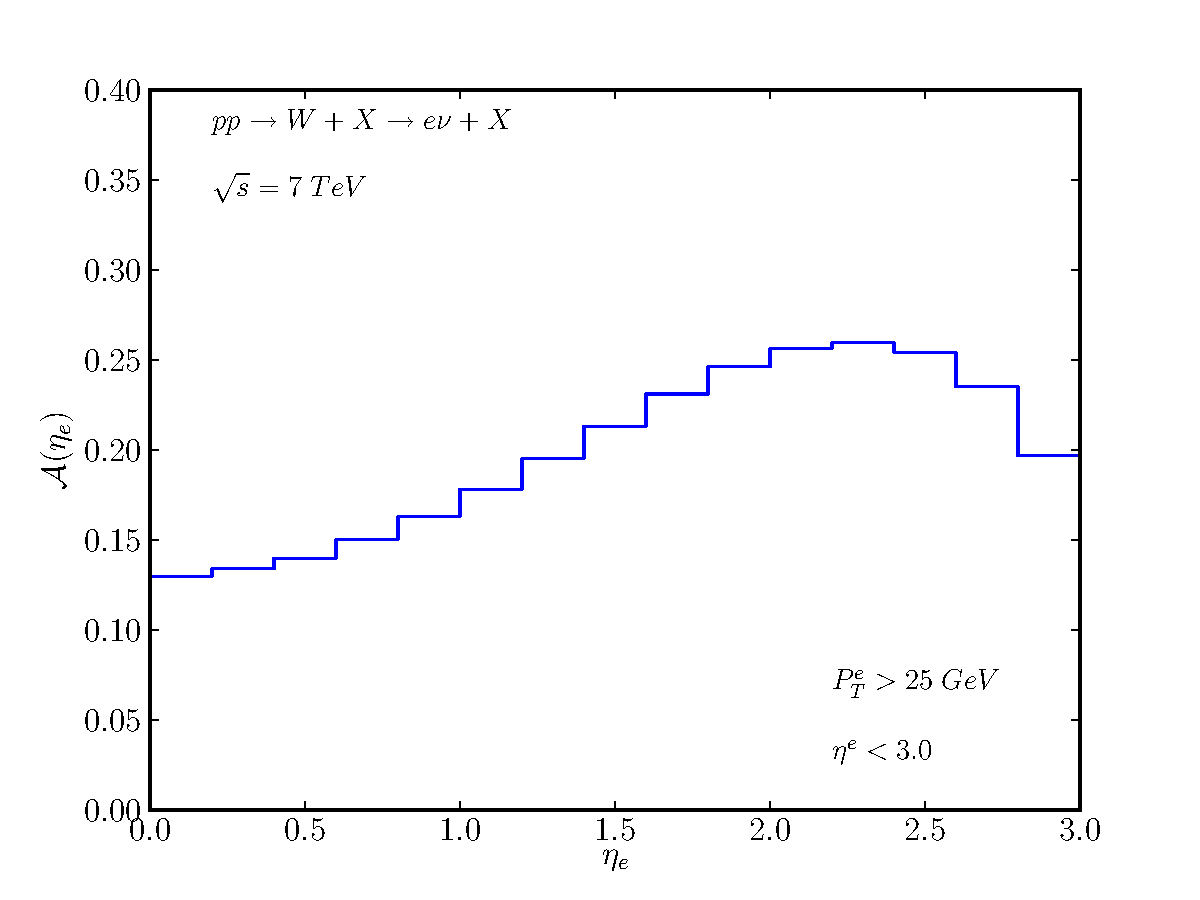
\includegraphics[width=0.8\textwidth]{lepton-asym}
  \caption{Electron charge asymmetry (simple).}
  \label{wbos:asym_simple}
\end{figure}

Unlike the \PW asymmetry , the electron asymmetry turns over at $\eta\approx
2.25$. Ths effect is due to the \ac{EWK} correlations in the leptonic decay of
the \PW boson.

In an experiment, the cross-section is not measured directly, instead what is
measured are the electron and positron yields.  The experimentally measured
asymmetry is given by \EquationRef{eq:AsymExp},
\begin{equation}
A_{exp}(\eta)=\frac{  \frac{dN}{d\eta}(\Pelectron) -
\frac{dN}{d\eta}(\APelectron) }{ \frac{dN}{d\eta}(\Pelectron) +
\frac{dN}{d\eta}(\APelectron) }
\label{eq:AsymExp}
\end{equation} 

To get from the experimentally measured asymmetry to the lepton charge
asymmetry, \EquationRef{eq:NumEve} must be used, which takes in to
account the experimental effects such as the luminosity (${\cal L}$), high
level trigger ($\epsilon_{HLT}$), offline efficiency ($ \epsilon_{off}$) and
the acceptance ($\epsilon_{acc}$).

\begin{equation}
\frac{dN}{d\eta} = {\cal L } \frac{d\sigma}{d\eta}  \epsilon_{HLT}
\epsilon_{off} \epsilon_{acc}
\label{eq:NumEve}
\end{equation} 
\todo{think about how this copes with a background...}
Since the asymmetry is a ratio, the luminosity, high level trigger and the
offline efficiency can be cancelled out assuming that they are not asymmetric
with respect to charge. 

The acceptance cannot be cancelled however, since it is a function of rapidity and 
these distributions will differ for \Pelectron and \APelectron.
The experimentally measured asymmetry can therefore be related to the
theoretical asymmetry by correcting for the acceptance.

\begin{align} 
A_{exp}(\eta) &= \frac{ \frac{dN}{d\eta}(\Pelectron) -
\frac{dN}{d\eta}(\APelectron) }{ \frac{dN}{d\eta}(\Pelectron) +
\frac{dN}{d\eta}(\APelectron) }\\   
              &= \frac{ \frac{d\sigma}{d\eta}(\Wpenu) -
\frac{\epsilon^{-}_{acc}}{\epsilon^{+}_{acc}} \frac{d\sigma}{d\eta}(\Wmenu) }{
\frac{d\sigma}{d\eta}(\Wpenu) + \frac{\epsilon^{-}_{acc}}{\epsilon^{+}_{acc}}
\frac{d\sigma}{d\eta}(\Wmenu) }
\label{eq:AsymExpCorr}
\end{align}

\section{Electron Charge Asymmetry Theoretical Predictions}

In this section predictions on the electron charge asymmetry are studied in detail.
The predictions are calculated using \ac{MCFM}\cite{mcfm} \ac{MC} tools interfaced with the
\ac{LHAPDF} package\cite{lhapdf}. 
\ac{LHAPDF} provides an interface to many different \ac{PDF} sets. For the
following predictions, \ac{PDF} from  the \ac{MSTW} and \ac{CTEQ} collaboration
are used.

\subsection{Uncertainty on Theoretical Predictions}
The theoretical predictions of the electron charge asymmetry will have an error
associated with the uncertainty on the \ac{PDF}.
The uncertainty on the \ac{PDF} originates from the experimental errors on the
data used in the global fits performed by each of the \ac{PDF} collaborations.

Each \ac{PDF} collaboration produces a set of \acp{PDFs} that include the
central value, or best fit to experimental data, and $2N$ error \acp{PDF}, where
$N$ is the number of free parameters used in the global fit.\cite{bourilkov}

The uncertainty on the observable, in this case the lepton asymmetry, is found
by producing $2N+1$ theoretical predictions, on for each member of the \ac{PDF}
set. The predictions are then used to approximate the \ac{PDF} uncertainty by
using the `master equation'.\cite{bourilkov} For the upper uncertainty,
\begin{equation}
\Delta A^{+}_{max}
= \sqrt{ \sum^{N}_{i=1} \left[ max( A^{+}_i-A_{0}, A^{-}_i-A_{0}, 0 ) \right]^{2}}
\end{equation}
and for the lower uncertainty,
\begin{equation}
\Delta A^{-}_{max}
= \sqrt{ \sum^{N}_{i=1} \left[ max( A_{0}-A^{+}_i, A_{0}-A^{-}_i, 0 ) \right]^{2}}
\end{equation}
where $A^{\pm}_{i}$ is the asymmetry prediction using the \ac{PDF} with the
positive/negative fluctuation of parameter $i$ and $A_{0}$ is the prediction
using the central value.

\begin{figure}[htbp]
  \centering
  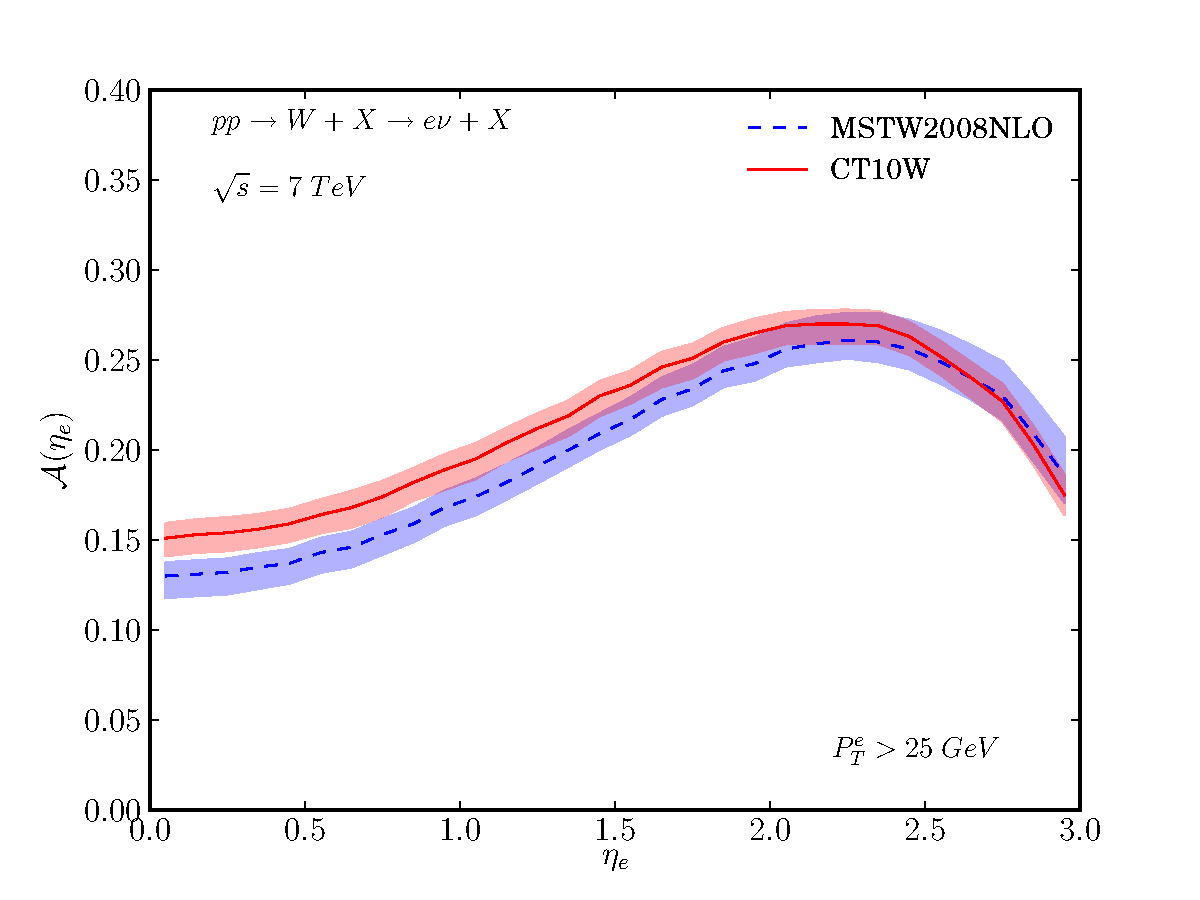
\includegraphics[width=0.8\textwidth]{asym-uncert}
  \caption{Electron charge asymmetry (uncert).}
  \label{fig:asym-uncert}
\end{figure}

\FigureRef{fig:asym-uncert} shows the electron charge asymmetry theoretical
predictions for a $\pT>\unit{25}{\GeV}$ with the \ac{PDF} uncertainties for the
\ac{PDF} sets MSTW08NLO\cite{MSTW} and CT10W\cite{CTEQ}. The uncertainties are
$68\%$ confidence level. The predictions are generated using the \ac{MCFM}
\cite{mcfm} generator.


